\chapter{Literature Review}

The main areas of research included papers and proposals on the design of
anonymity networks and those covering the subject of traffic analysis.
Particular attention has been paid to encryption as it is the primary function
by which these systems operate and a good understanding is necessary for the
development of an appropriate traffic analysis method.

\section{Encryption}

Since the creation of language, the interception of messages by hostile forces
has compelled the development of secretive communications. This deliberate
transformation of a message, so that only the intended recipient can understand
it, is known as encryption. The process of examining these obfuscated messages
and attempting to reverse the transformation is known as cryptanalysis
\parencite{Schneier:1996uq}. These fields have been locked in an arms race
ever since, each side continually advancing their capabilities in an attempt to
gain ground.

Apart from One Time Pads, no encryption methodology has ever proven to be
unbreakable \parencite{Shannon:1948p6583}. This means that all remaining
cryptographic methods are a way of transforming information, so that for an
attacker the difficulty in reversing this transformation is too costly to make
it worthwhile. The invention of robots and computers was precipitated by the
need to break encryption methods of increasing complexity and at the same time
has lead to the increasing complexity of encryption algorithms
\parencite{Kahn:1974:C}.

Historically, all encryption methods have required an interaction between those
communicating. A meeting to exchange the secret communications key, or a
courier to deliver the encryption device. This made anonymous communications
difficult, especially when using digital communications technologies.  In
\citeyear{Jevons:1874vn}, \citeauthor{Jevons:1874vn}, perhaps
unknowingly, uncovered the mathematical techniques that would allow for public
key cryptography in his publication \citetitle{Jevons:1874vn}. He recognised
that certain mathematical operations yielded products that were impossible or
difficult to reverse in order to uncover the factors used.

The possibility of public key cryptography, or non-secret encryption was
conceived by James H. Ellis in \citeyear{Ellis:1970p3249} and later developed
into both a method for sharing secret encryption keys by Malcolm J. Williamson
in 1974 \parencite{Singh:1999:CBE} and a method for asymmetric encryption
\parencite{Cocks:1973p3265}.

These papers were not published at the time due to their military
classification, allowing these methods to be reinvented independently
\parencite{Singh:1999:CBE}. The method for key sharing developed by Ellis
later became known as the Diffie-Hellman key exchange
\parencite{Diffie:1976p585}, while the method for asymmetric encryption is now
known as RSA encryption, taking its name from the initials of its creators,
Rivest, Shamir and Adleman \parencite{Rivest:1978p708}. Figure
\ref{key-exchange} shows how discrete logarithms are used in the Diffie-Hellman
algorithm to generate a shared encryption key.

\begin{figure}[H]
  \centering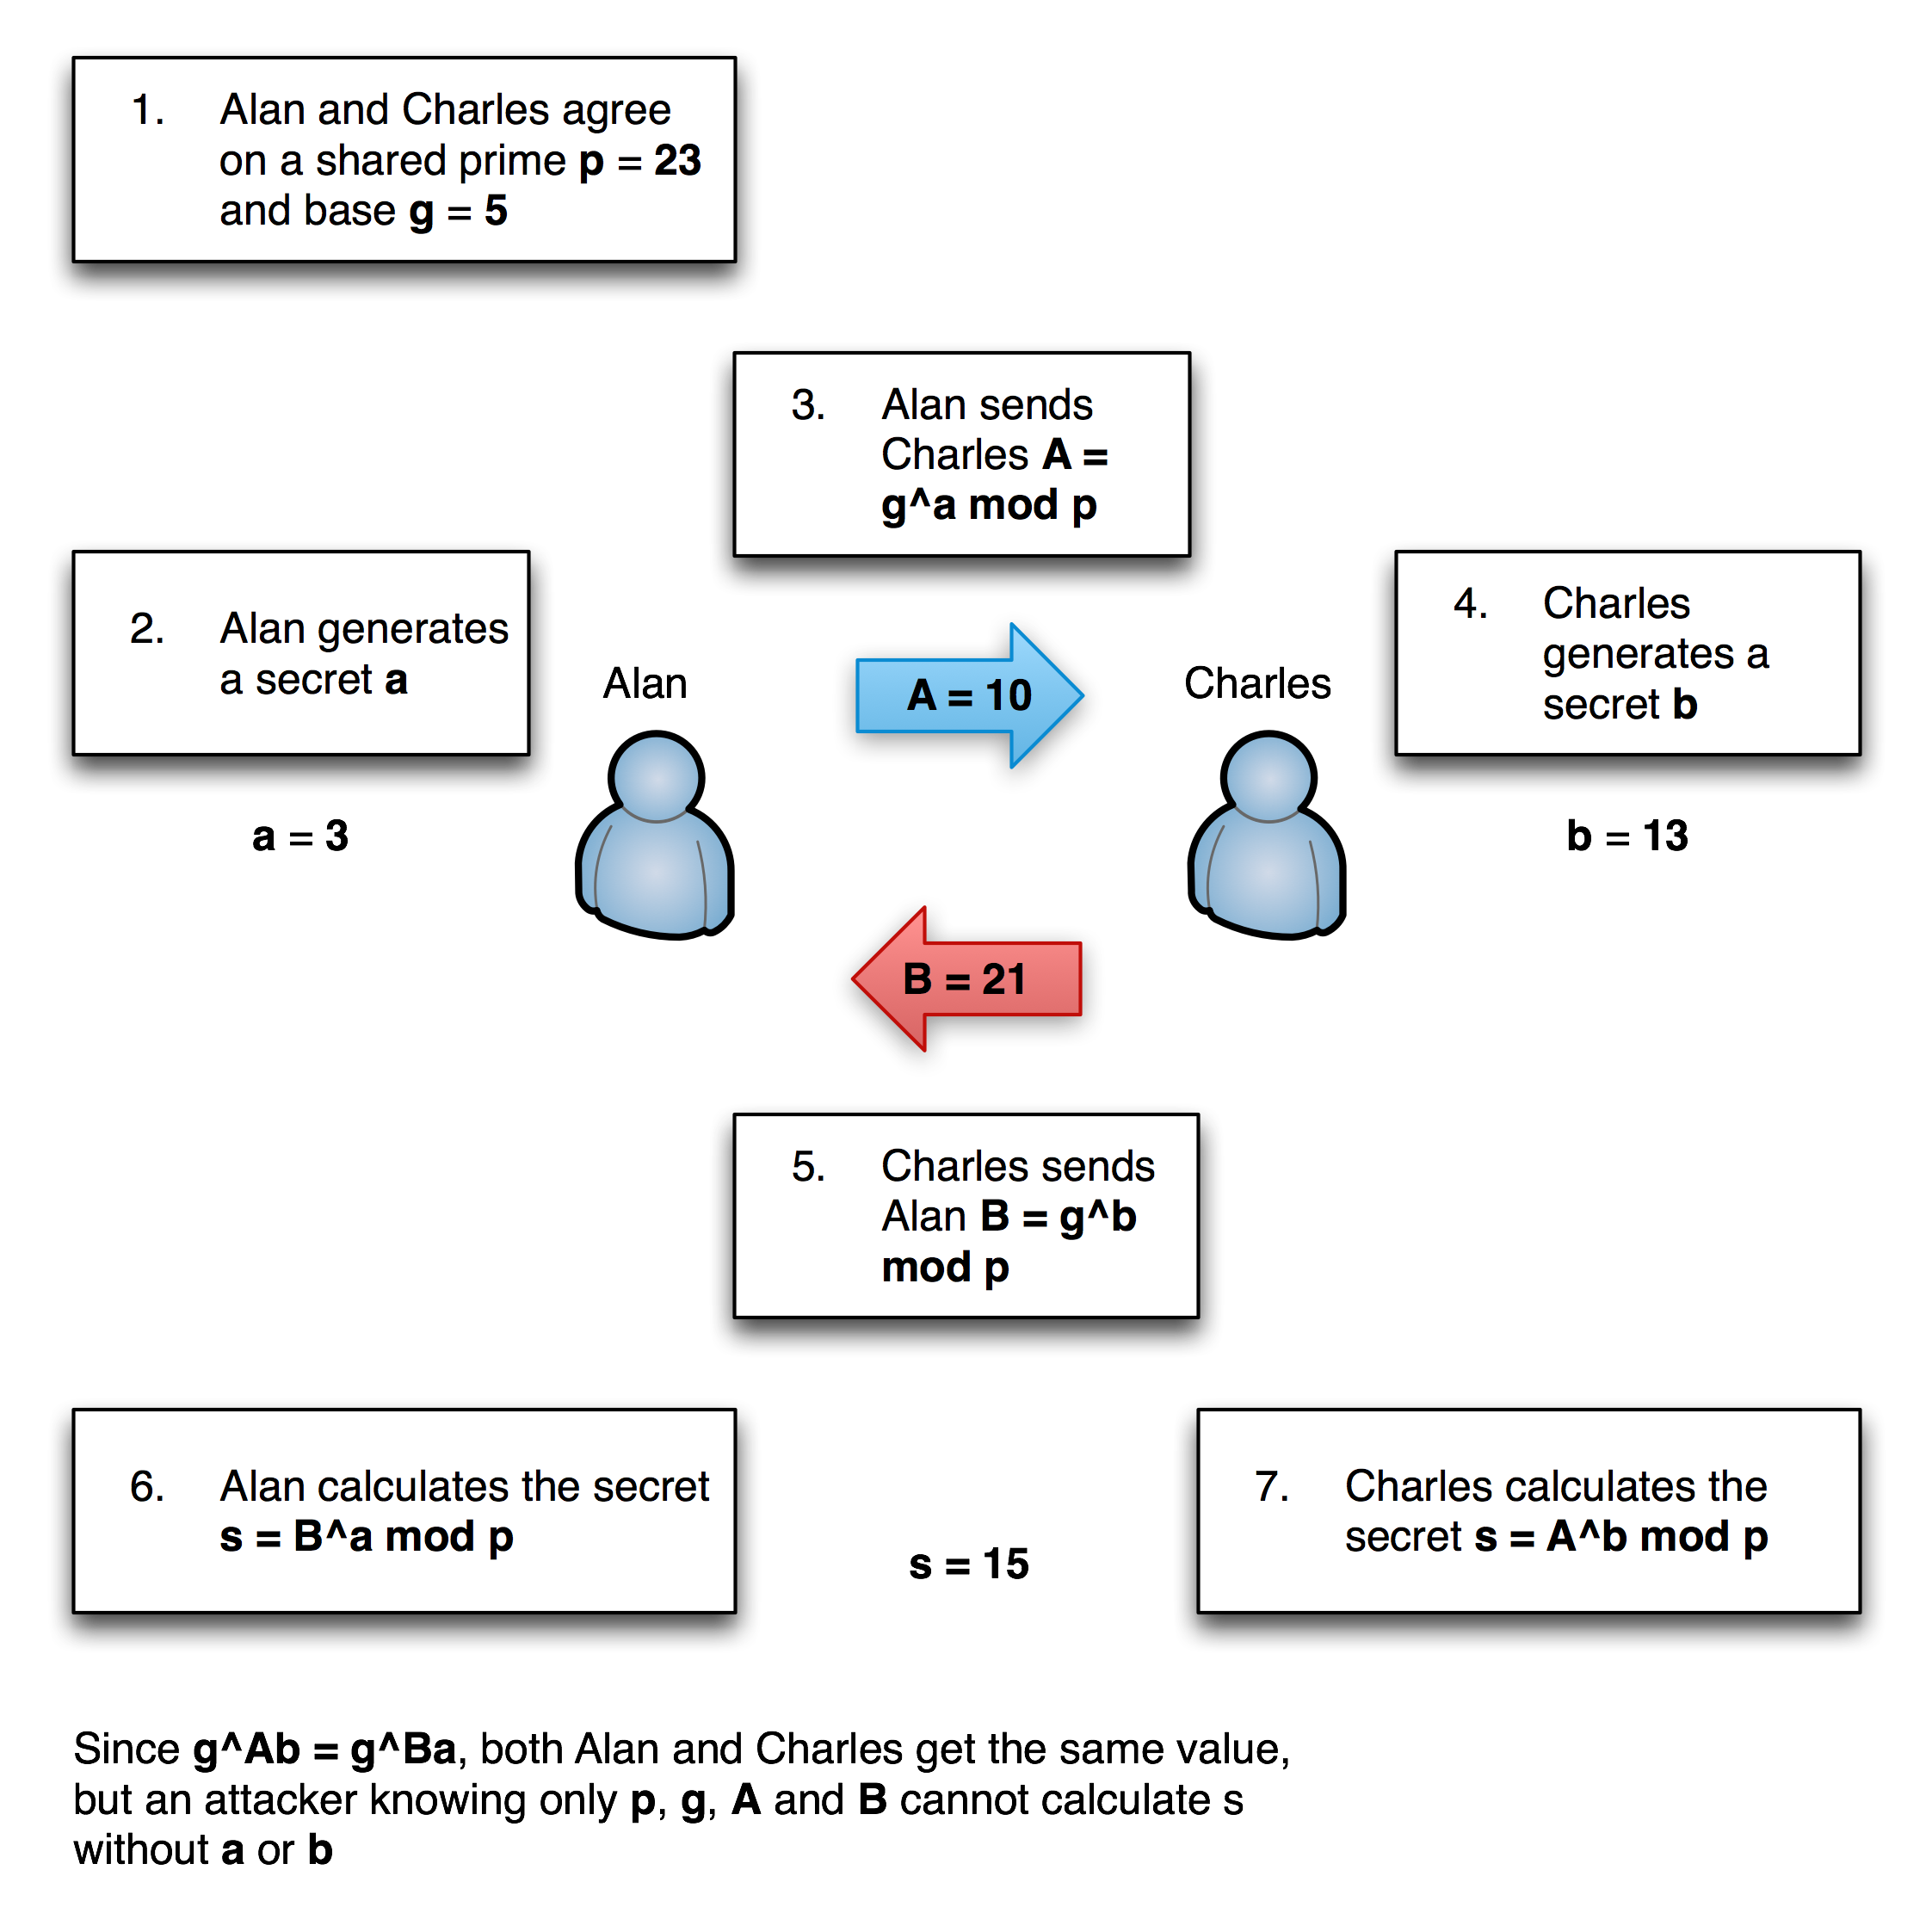
\includegraphics[width=\linewidth]{key-exchange}
  \caption{Diffie-Hellman Key Exchange}
  \label{key-exchange}
\end{figure}

% How to relate back to Tor:
% What algorithm does Tor use
% How does encryption resist traffic analysis
% Modern encryption algorithms ensure resistance to frequency analysis by making sure every character in a message appears as likely as every other character. To an observer, this means that encrypted messages appear to be indistinguishable to noise.

While these early public key encryption algorithms are still in use, newer
implementations have appeared which make improvements including
\textcite*{ElGamal:1985p529} and \textcite{Cramer:1998p3186}. Attempts to make
these encryption algorithms more difficult to break have involved the use of
increasingly complex mathematical problems such as elliptic curves
\parencite{Miller:1986p2966,Koblitz:1987p3109} and probabilistic functions
\parencite{Paillier:1999p3152}. Many of these encryption algorithms are
available in modern encryption protocols.

Early proposals for digital networks included extensive usage of encryption
technology. \textcite{Baran:1964p384} suggested that future digital military
networks should use encryption for all messages, even those that did not
require any secrecy. He cited benefits such as tamper resistance, message
secrecy and resistance to traffic analysis, although this system was never
implemented. The Internet, was developed without encryption features
\parencite{website:internet}.

Early work in encrypted Internet communications includes the Secure Network
Programming (SNP) Applications Programming Interface (API)
\parencite{Woo:1994p2532}. This was a simple framework providing numerous
encryption, signing and authentication methods. The Secure Sockets Layer (SSL)
is an encryption layer which provided end-to-end communications secrecy on the
Internet \parencite{website:SSL}. A primary feature of SSL is the ability to
exchange secret keys using public key algorithms.

This proposed standard went through a number of revisions, with early versions
suffering security flaws \parencite{Wagner:1996p385}. SSL is now known as
Transport Layer Security (TLS), with the latest version 1.2 being released
August 2008 \parencite{website:TLS}. TLS addresses some issues in SSL and
provides a number of enhancements, but is not compatible with SSL.

The Hypertext Transfer Protocol Secure (HTTPS) provides encryption using both
the TLS and SSL protocols \parencite{website:HTTPS} and is available in almost
all modern web browsers including Firefox
\parencite{website:firefox-encryption}, Safari
\parencite{website:safari-features} and Internet Explorer
\parencite{website:microsoft-tls}. Tor provides encryption through usage of the
TLS protocol.

\section{Anonymous and Censorship Resistant Networks}

The first anonymous network system MixNet, was described in
\textcite{Chaum:1981p296}. This proposal makes essential usage of public key
encryption to prevent eavesdroppers from obtaining message delivery information.
Senders in the network communicate with a centrally located server known as a
mix, delivering a message with the address of the intended recipient. The mix
server discards any information about the sender and delivers it to the final
destination. Figure \ref{chaums-mix-network} depicts the process of message
delivery in Chaum's MixNet. Chaum's proposal also allowed for the chaining of
multiple mix servers together to form a cascade.

\begin{figure}[H]
  \centering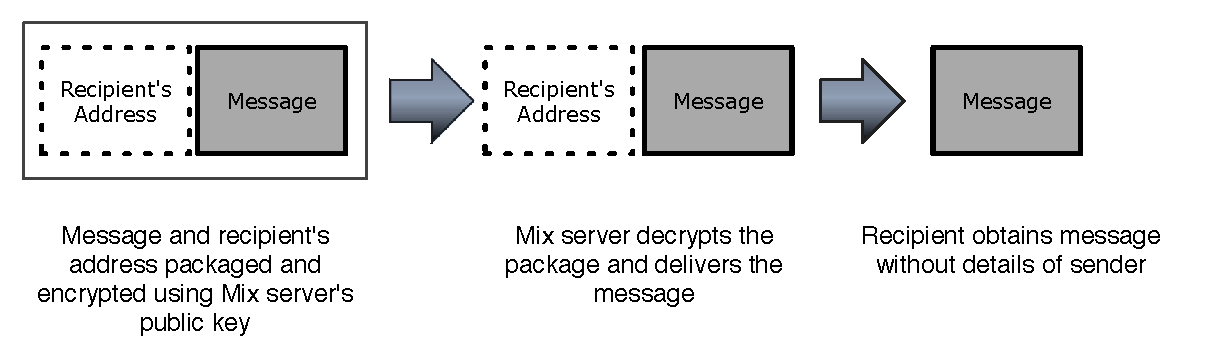
\includegraphics[width=\linewidth]{chaums-mix-network}
  \caption{MixNet Message Delivery}
  \label{chaums-mix-network}
\end{figure}

Since the inception of MixNet, numerous anonymous networks have been proposed,
each design being influenced by diverse motivations for obtaining anonymity.
These include:

\begin{itemize*}
  \item Anonymous remailers such as Babel \parencite{Gulcu:1996p1662} and
    Mixminion \parencite{Danezis:2003ys}.
  \item Networks that provide mathematically provable anonymity
    \parencite{Chaum:1988p5869,Waidner:1989p5870,Berman:2004p303}.
  \item Anonymity that degrades gracefully when subject to attack, so called
    robust anonymity \parencite{Waidner:1989p5870,Jakobsson:1998p5137}.
  \item Anonymous publishing in Freedom \parencite{Goldberg:1999p2231} and
    Freenet \parencite{Clarke:2001p2435}.
  \item Peer to Peer (P2P) anonymity such as MorphMix
    \parencite{Rennhard:2002p4559}, Tarzan \parencite{Freedman:2002kx} and P5
    \parencite{P5Sherwood:2005p5872}.
  \item Censorship resistance in aChord and gnuNet \parencite{Hazel:2002p6929},
    Infranet \parencite{Feamster:2002p307} and of course Tor.
\end{itemize*}

This is by no means an exhaustive list, for an excellent survey of anonymous
networks consult \textcite{Danezis:2008p346}.

Although this research has yielded a variety of designs, all anonymous
networks essentially operate on all or some of the following principles:

\begin{itemize*}
  \item Encrypting traffic to prevent eavesdropping.
  \item Providing covering traffic through a network of active users or by
    generating it automatically.
  \item Normalizing message delivery so that individual communication patterns
    are not identifiable.
\end{itemize*}

In theory, the normalization techniques used by anonymous networks should make
them readily distinguishable from non anonymous communications.

\subsection{The Second Generation Onion Router (Tor)}

Tor was first described in \citetitle{Dingledine:2004p314}
\parencite{Dingledine:2004p314}. This new generation of onion router was
designed with a number of defences for common traffic analysis attacks and
weaknesses discovered in other proposals. With a focus on deployability,
usability, flexibility and simple-design \parencite[3-4]{Dingledine:2004p314}
as well as a successful implementation, it has seen wider deployment than most
other anonymous networks.

Like MixNet, public key cryptography is combined with intermediate servers
responsible for message delivery to provide a degree of anonymity. In Tor,
these mixes are known as relays and are typically chained together to
construct a circuit. Clients connect to the Tor network by communicating
with a special relay known as a bridge, which constitutes the first
relay in a circuit. Traffic is repeatedly delivered through relays until it
reaches another special relay known as an exit node, where it is
delivered unencrypted to the final destination. Figure \ref{tor-network} shows
this typical usage of the Tor network.

\begin{figure}[H]
  \centering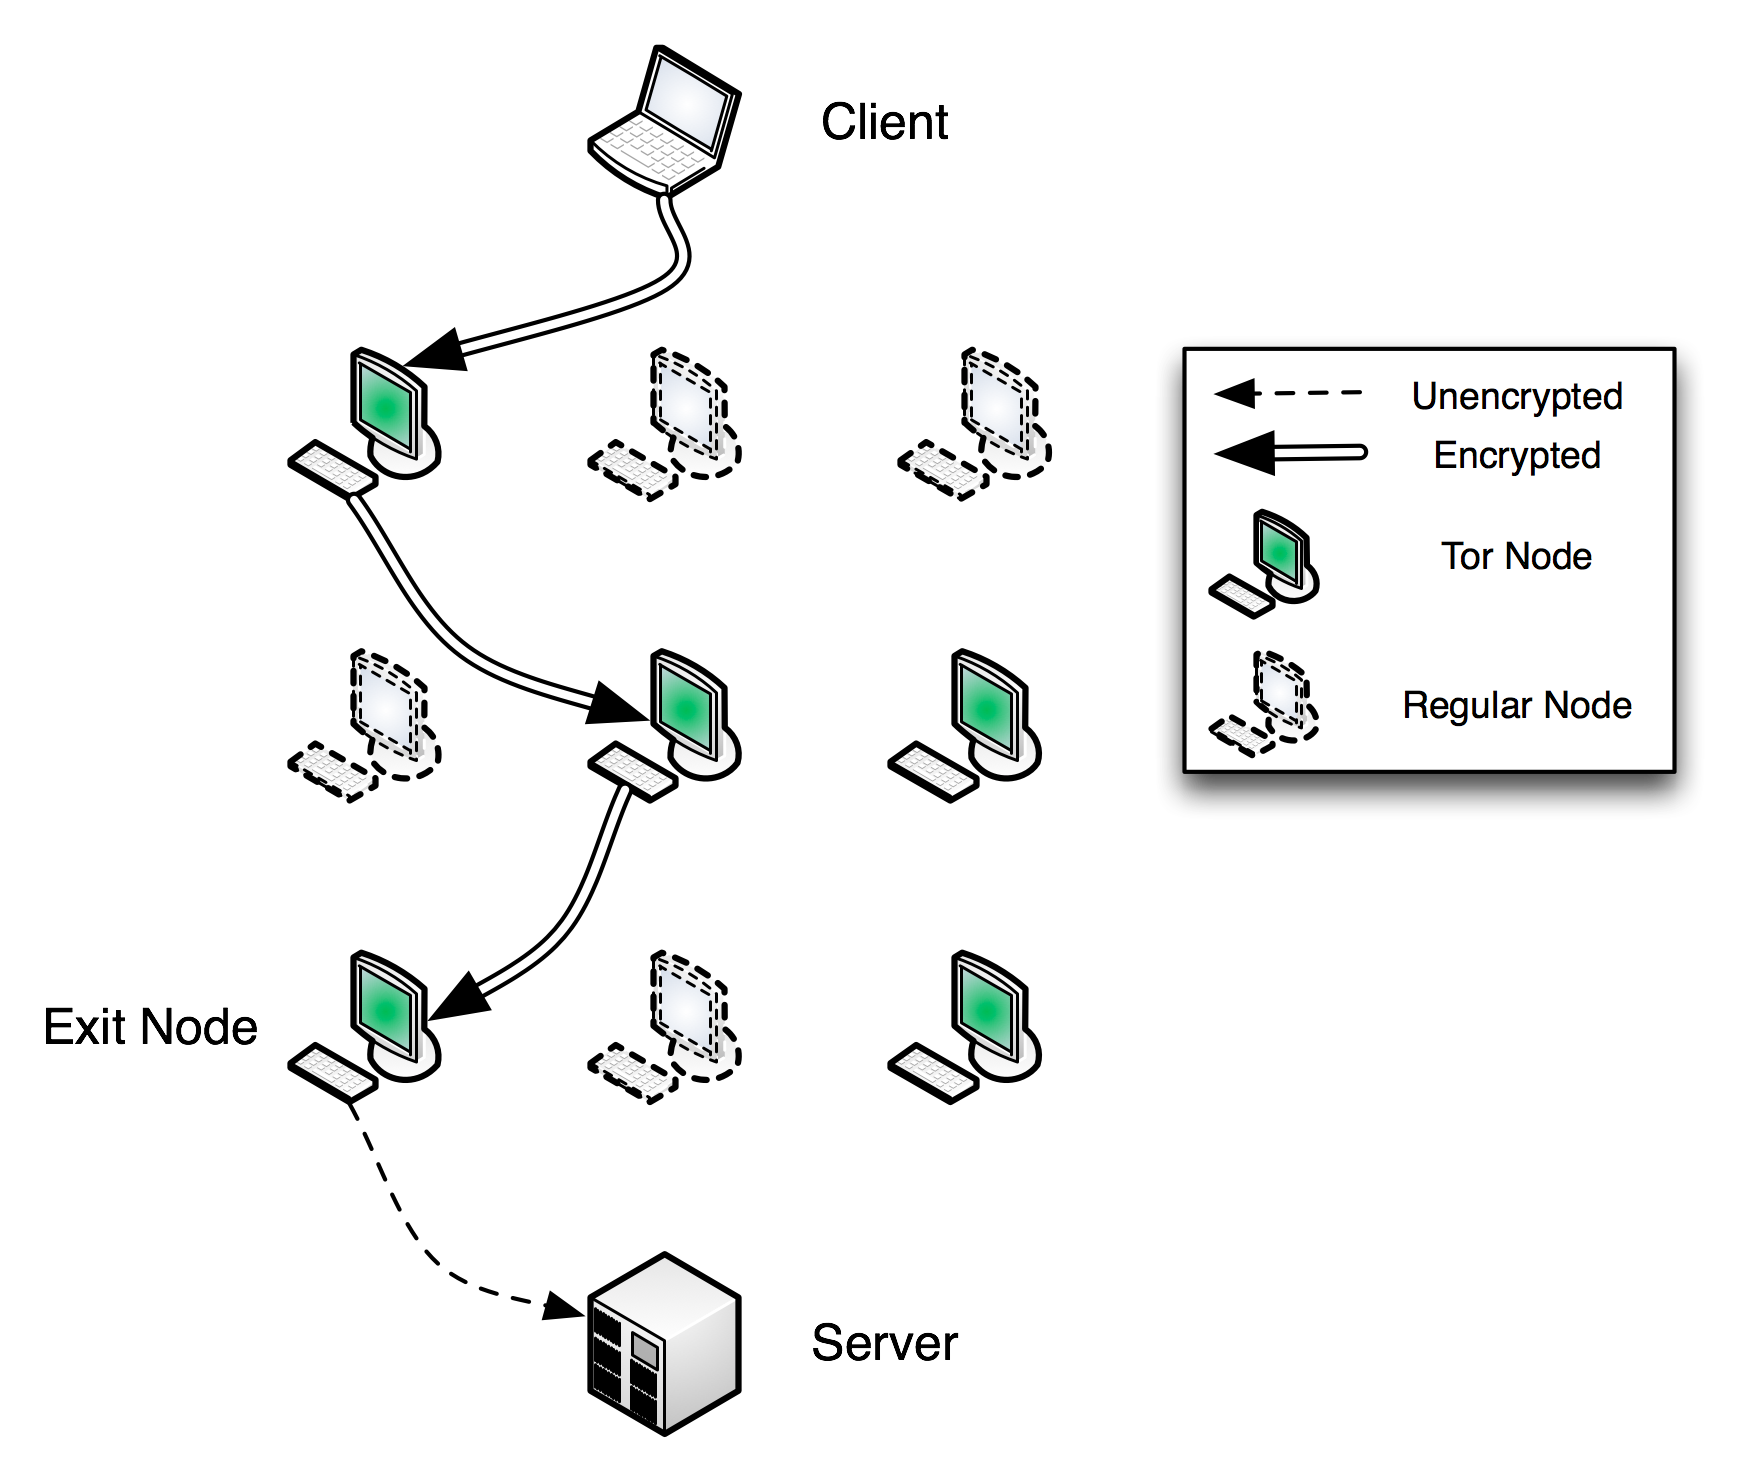
\includegraphics[width=\linewidth]{tor-network-diagram}
  \caption{The Tor Network}
  \label{tor-network}
\end{figure}

Messages delivered through the Tor network are encrypted multiple times using a
variation of onion routing \parencite{Michael:2001} known as telescopic onion
routing. Circuits are built incrementally, obtaining a session key from each
successive relay in the circuit and encrypting messages so that intermediate
relays are unable to decrypt the message. Since circuits can take some time to
build, they are pre-emptively created at regular intervals
\parencite[5]{Dingledine:2004p314}. Although Tor does not support many of the
traffic normalization techniques that provide strong anonymity, messages passed
through the Tor network are packaged in cells of a fixed size of 512 bytes
\parencite[5]{Dingledine:2004p314}. Tor also provides application level filters
that remove identifying features from common application protocols.

After it was noticed that Tor was being used to circumvent censorship as well
as for anonymity, a publication was released which attempts to identify the
issues that need to be addressed in order for Tor to provide some level of
censorship resistance \parencite{Dingledine:2008p1542}. Although this paper
foresees future attacks such as the one contained in this proposal, it mostly
tackles social issues of censorship resistance.

\section{Traffic Analysis}

Research into Tor weaknesses has included the use of hostile exit nodes to
capture private information \parencite{website:tor-password-leak}, attacks that
take advantages of web based technologies such as Javascript and Flash to reveal
user's identities \parencite{Abbott:2007p298} and a number of identity revealing
traffic analysis techniques
\parencite{Murdoch:2005p325,Abbott:2007p298,Evans:2009p315}.
\citeauthor{McLachlan:2009p197} reveals a method for identifying bridge
operators in \textcite{McLachlan:2009p197} using the Tor protocol directly.  It
is believed that this is the first proposal of a traffic analysis technique for
classification of Tor network streams.

When considering the use of traffic analysis for classification of Internet
communications, three techniques are used. These are: exact matching, heuristic
matching and machine learning \parencite{Zhang:2009p1188}. Exact matching
techniques recognise properties of communications that mirror known protocols
and communication patterns. This might include the port an application uses or
the format of its payload. Since Tor employs strong encryption and communicates
using known and commonly used protocols, exact matching techniques would prove
ineffective for classification. Heuristic matching looks for patterns in
conversations to determine communications patterns and infer relationships,
while machine learning involves the use of statistics to train computer
algorithms to classify traffic. Both heuristic and machine matching techniques
are suitable for traffic analysis of anonymous networks because they do not
rely on analysing the content of messages.

\subsection{Heuristic Techniques}

The increasing burden of peer to peer (P2P) applications on campus networks,
and their shift to encryption motivated the development of heuristics based
techniques for identifying P2P traffic. Early techniques include identifying
known properties of P2P networks such as often communicating using both the UDP
and TCP protocols simultaneously and using a solitary connection to transfer
high volumes \parencite{Karagiannis:2004p6400}. This paper also reduced the
number of false positives by eliminating packets that matched known
communications protocols.

Similar techniques have been developed in \textcite{Perenyi:2006p6325} and
\textcite{John:2008p1376}, both of which attempt to improve matching accuracy
through early elimination of false positives and by expanding the scope of
matching parameters. In \textcite{Oneil:2004p6451} the same heuristics are used
to identify P2P nodes before applying a secondary heuristic to identify
‘supernodes’ which are a subset of all P2P nodes.

Classifying traffic based on system roles is a key feature of the technique
that appears in \citetitle{Karagiannis:2005p6359}
\parencite{Karagiannis:2005p6359}. By analysing communications at the host
level then at increasing levels of granularity, a greater level of accuracy is
achieved.

The use of Traffic Dispersion Graphs or TDGs to identify P2P traffic appears in
\textcite{Iliofotou:2008p6373} and \textcite{Iliofotou:2009p6461}. Once traffic
flows are represented in a TDG, mathematical properties of the flow can be
analysed to make positive identifications.

Viruses have also posed a problem for network administrators, often
over-utilizing network resources and using the network to infect new machines.
A technique for identifying various worms was proposed in
\textcite{Lazarevic:2003p6450}. Worms often attempt to hide their communications
from network administrators to avoid detection, presenting the same problems of
identification as Tor network traffic.

\subsection{Machine Learning Techniques}

\subsubsection{Expectation-Maximisation}

The first use of machine learning to categorise traffic flows appears in
\textcite{McGregor:2004p3826}. A detailed analysis of the attributes that can
be used for machine learning and an attempt at coarse grained classification
using an expectation-maximisation (EM) algorithm are demonstrated. The
expectation-maximisation algorithm is a method for finding probabilistic
estimates of parameters in a statistical model \parencite{UW:2010p7083}. The
same technique is also demonstrated in \textcite{Soule:2004p3817} using
histograms for finer grained classification.  The EM algorithm is again used in
\textcite{Zander:2005p6212} and \textcite{Erman:2006p3825}, with the latter
comparing EM favourably against a Na\"{i}ve Bayes classifier.

\subsubsection{Na\"{i}ve Bayes}

\textcite{Moore:2005p3827} use a supervised Na\"{i}ve Bayes to classify traffic
flows that have previously been sorted into groups by analysing the flow
content. This paper focuses on many of the most commonly used Internet
protocols while \textcite{Bonfiglio:2007p6453} uses the technique for
identifying traffic belonging to the Skype application.

\textcite{Herrmann:2009p1189} uses Bayesian networks to fingerprint visited
websites accessed through Privacy Enhancing Technologies (PET), including Tor.
This technique performed poorly when applied to the Tor network, but it
suggests that Tor traffic has particular characteristics that distinguish it
from many existing PETs. It makes a particularly useful observation: ``The most
frequent packet sizes in the Tor traffic dumps are, in descending order, 1500,
−52, −638, 52, 638 and 1150 bytes, accounting for 87.6 \% of all Tor packets.''

\subsubsection{Markov Models}

Hidden Markov Models (HMM) are a statistical modelling technique useful
for classification of systems with an unobservable state
\parencite{Rabiner:1990p1153}. HMMs are first used as a traffic analysis
technique in \citetitle{Wright:2004p3860} \parencite{Wright:2004p3860}. The
primary identification characteristics for use with this algorithm are packet
size and inter-packet arrival times. With refinement this algorithm is used
with increasing accuracy in \textcite{Wright:2006p322} and
\textcite{Dainotti:2008p1435}.

In \textcite{Bernaille:2005p6205} a spectral clustering algorithm is used to
discover distinguishing characteristics of traffic flows, rather than with a
specific set of classification goals. This information is used to build HMMs
for the purpose of traffic classification.

Since HMMs model particular behaviours, they can be used to recognize
deviations from normal behaviour as shown in
\textcite{EstevezTapiador:2003p7201}. Motivated by
\citeauthor{EstevezTapiador:2003p7201}, \textcite{Munz:2010p7085} uses TCP
flags and the position of individual packets in a stream to train an Observable
Markov Model for traffic classification, achieving greater classification
accuracy than \citeauthor{Bernaille:2005p6205}.

\subsubsection{Clustering}

Clustering algorithms group observations into subsets based on similar
characteristics, they are a form of unsupervised learning technique designed to
discover organization in unlabelled data sets. They have been the basis of a
number of traffic classification techniques with the K-Means clustering
technique being the most prominent.  K-Means cluster analysis appears in
\textcite{Bernaille:2006p2366}, \textcite{Erman:2007p3764} and
\textcite{Erman:2007p6206}. The use of the Density Based Spatial Clustering of
Applications with Noise (DBSCAN) algorithm appears in
\textcite{Erman:2006p3766}, alongside K-Means and Autoscan algorithms.

\subsubsection{Other Techniques}

Other algorithms used for traffic classification include Nearest Neighbour and
Linear Discriminant Analysis \parencite{Roughan:2004p3823}, Normalized
Threshold \parencite{Crotti:2007p3824}. The use of the Gaussian Mixture Model
to identify applications and identities inside SSH tunnels was demonstrated in
\textcite{Dusi:2008p6254}. Several algorithms are compared in
\textcite{Alshammari:2009p7474}, finding the C4.5 algorithm the most accurate
for identifying Skype and SSH traffic.

\subsubsection{Comparing Techniques}

It is difficult to say what machine learning technique is the most effective as
no consensus has been reached, the literature covers a wide variety of
techniques each with vastly different goals and no two techniques can be
directly compared as the data used for analysis has not been disclosed
\parencite{Kim:2007p3867}. However some attempt has been made at comparison in
\textcite{Williams:2006p3849} which suggests that the C4.5 algorithm has the
greatest performance and accuracy when compared to a number of Bayesian
algorithms. \textcite{Mohd:2009p6484} compares thirty machine learning
algorithms  to find random tree, IBI, IBK and random forest algorithms
obtaining the greatest classification accuracy.

An excellent meta study on traffic analysis techniques is presented in
\textcite{Nguyen:2008p3837}. This paper compares many of the published papers,
the techniques used, criteria analysed and how effectively they meet stated
goals.
